
\section{Uniform Circular Motion\footnote{
1990-93 Dept. of Physics and Astronomy, Dickinson College. Supported by FIPSE
(U.S. Dept. of Ed.) and NSF. Portions of this material have been modified locally
and may not have been classroom tested at Dickinson College.
}}

\makelabheader %(Space for student name, etc., defined in master.tex or labmanual_formatting_commands.tex)

\textbf{Objective }

To explore the phenomenon of uniform circular motion and the acceleration needed
to maintain it.

\textbf{Overview} 

You have recently studied projectile motion. In this unit we are going to explore
another phenomenon in two dimensions, uniform circular motion. In particular,
you will develop a mathematical description of the centripetal acceleration
that keeps an object moving in a circle. You will start by watching a toy ``airplane''
suspended from a string fly in a circle.

\textbf{Apparatus}

\begin{itemize}
\item The ``airplane.''
\item A movie scaling ruler or meter stick.
\item A video analysis system(\textit{Tracker}). 
\item Graphing software (\textit{Excel}).
\end{itemize}
\textbf{Activity 1: Observing an Airplane Undergoing Circular Motion} 

(a) Put on your safety glasses and wear them until your instructor announces
that they can be removed. Turn on the engine of the airplane suspended from
the string. Be careful to stay clear of the propeller. Launch the airplane into
circular motion by giving it a gentle push. If it doesn't quickly settle into
steady circular motion, catch it and try launching it in the opposite direction.
Sketch the motion and describe it in words below. 
\vspace{30mm}

(b) How would you describe the speed of the airplane? How would you
describe the velocity? Would you say that this is accelerated motion? Why?
\vspace{20mm}

(c) What is the definition of acceleration? (Remember that acceleration is a vector!)
\vspace{20mm}

(d) Are velocity and speed the same thing? Is the velocity of the airplane constant?
(Hint: Velocity is a vector quantity!)
\vspace{20mm}

(e) In light of your answers to (c) and (d), would you like to change your answer
to part (b)? Explain.
\vspace{20mm}

The two-dimensional motion of the airplane is too fast to observe carefully
so we will use a video system to record the motion of the airplane and to analyze
the movie frame-by-frame. You will use the video analysis system to investigate
the direction of the velocity of the circling airplane and the direction of
its acceleration.

\textbf{Activity 2: Analyzing Circular Motion }

(a) Make a movie of the airplane in flight by following these steps. 

\begin{enumerate}
\item Open \textbf{Camera} and turn on the video camera as explained in \textbf{Appendix \ref{tracker}: Video Analysis Using Tracker}. Center the field of view on the region where the
plane will fly. This region should be at least 1 meter from the camera to get a
large enough area for the flight of the plane. Mount a ruler or meter stick
somewhere in the field of view where it won't interfere with the motion. This
ruler will be used later to determine the scale. 
\item Launch the airplane into circular motion and wait until it settles into steady,
circular flight. Record several revolutions of the airplane and save the movie as the file Airplane. See \textbf{Appendix \ref{tracker}: Video Analysis Using Tracker} for details on making the movie.
\end{enumerate}
(b) Determine the position of the airplane during one complete revolution using \textit{Tracker}.  The resulting file should contain three columns with the values of time, $x$-position, and $y$-position for one complete revolution. 

(c) Within \textit{Tracker}, make a graph of the trajectory of the airplane during one full revolution.
This can be done by plotting $y$ vs $x$. When you make your plot make sure the $x$ and $y$ 
axes cover the same size range; otherwise you will distort the path of the airplane. Double click 
on the graph to produce a larger version. Print the graph and attach a copy to this unit.

\begin{enumerate}
\item Is the motion circular? What is your evidence?\vspace{10mm}

\item Draw vectors for the position vector and the velocity vector at one point on
the trajectory. How are the position vector and the velocity vector related? How is the velocity vector
related to the path of the airplane?\vspace{30mm}

\item What would happen to the path of the plane if you cut the string? Explain.\vspace{20mm}

\end{enumerate}

\newpage
(d) Launch the airplane into uniform circular motion. You are going to investigate
what happens to the trajectory after the string is cut. Be sure you are wearing
your eye protection. After the plane settles into steady, circular flight start
recording a movie of the plane. After it completes one revolution use the scissors
to cut the string just above the horizontal metal bar. BE CAREFUL to avoid letting
the plane strike anyone or any object except the floor. Halt recording and save
the movie.

(e) Make a plot of the trajectory of the airplane after the string was cut and
for at least one full revolution before. Is the trajectory circular before the
string was cut? Does the trajectory of the plane after the string was cut agree
with the prediction you made earlier? Explain. Print the graph and attach a
copy to the unit.
\vspace{20mm}

\textbf{Using Vectors to Diagram How Velocity Changes} 

By now you should have concluded that since the direction of the motion of an
object undergoing uniform circular motion is constantly changing, its velocity
is also changing and thus it is accelerating. We would like you to figure out
how to calculate the direction of the acceleration and its magnitude as a function
of the speed v of an object such as a ball as it revolves and as a function
of the radius of the circle in which it revolves. In order to use vectors to
find the direction of velocity change in circular motion, let's review some
rules for adding velocity vectors.

\vspace{0.3cm}
{\par\centering 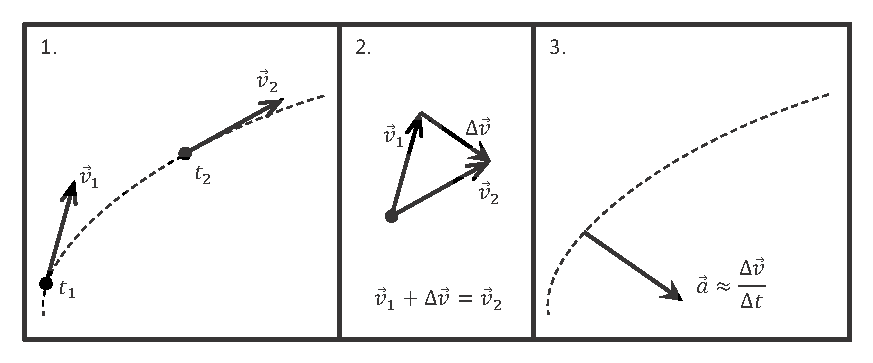
\includegraphics{circ_motion/circ_motion_fig1_new.eps} \par}
\vspace{0.3cm}

\begin{enumerate}
\item To Draw Velocities: Draw an arrow representing the velocity, \( {\bf v}_{1} \), of
the object at time \( t_{1} \). Draw another arrow representing the velocity,
\( {\bf v}_{2} \), of the object at time \( t_{2} \). 
\item To Draw Velocity Change: Find the change in the velocity \( \Delta 
{\bf v}
= {\bf v}_{2}  - {\bf v}_{1} \) during the time interval described
by \( \Delta  t = t_{2} - t_{1} \). Start by using the rules of
vector sums to rearrange the terms so that ${\bf v}_{1} + \Delta {\bf v}
= {\bf v}_{2}$. Next place the tails of the two velocity vectors together
halfway between the original and final location of the object. The change in
velocity is the vector that points from the head of the first velocity vector
to the head of the second velocity vector. 
\item To Draw Acceleration: The acceleration equals the velocity change 
\( \Delta  {\bf v}\)
divided by the time interval $\Delta t$ needed for the change. Thus, \textbf{a} is in
the same direction as \( \Delta  \textbf{v}\) but is a different length (unless
 \( \Delta  t = 1\)). Thus, even if you do not know the time interval, you
can still determine the direction of the acceleration because it points in the
same direction as \( \Delta  \)\textbf{v}. 
\end{enumerate}
The acceleration associated with uniform circular motion is known as centripetal
acceleration. You will use the vector diagram technique described above to find
its direction. 

\pagebreak[2]
\textbf{Activity 3: The Direction of Centripetal Acceleration }

(a) Determine the direction of motion of the ball shown below if it is moving
counter-clockwise at a constant speed. Note that the direction of the ball's
velocity is always tangential to the circle as it moves around. Draw an arrow
representing the direction and magnitude of the ball's velocity as it passes
the dot just before it reaches point A. Label this vector \textbf{v}\( _{1} \). 

%\vspace{0.3cm}
{\par\centering 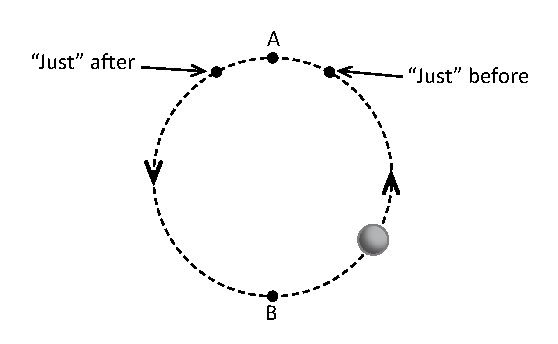
\includegraphics{circ_motion/circ_motion_fig2_new.eps} \par}
%\vspace{0.3cm}

(b) Next, use the same diagram to draw the arrow representing the velocity of
the ball when it is at the dot just after it passes point A. Label this vector
\textbf{v}\( _{2} \).

(c) Find the direction and magnitude of the change in velocity as follows. In
the space below, make an exact copy of both vectors, placing the tails of the
two vectors together. Next, draw the vector that must be added to vector \textbf{v}\( _{1} \)
to add up to vector \textbf{v}\( _{2} \) ; label this vector \( \Delta  \)\textbf{v}.
Be sure that vectors \textbf{v}\( _{1} \) and \textbf{v}\( _{2} \) have the
same magnitude and direction in this drawing that they had in your drawing in
part (a)!
\vspace{30mm}

(d) Now, draw an exact copy of \( \Delta  \)\textbf{v} on your sketch in part
(a). Place the tail of this copy at point A. Again, make sure that your copy
has the exact magnitude and direction as the original \( \Delta  \)\textbf{v}
in part (c).
\vspace{20mm}

(e) Now that you know the direction of the change in velocity, what is the direction
of the centripetal acceleration, \textbf{a}\( _{c} \)?
\vspace{20mm}

(f) If you redid the analysis for point B at the opposite end of the circle,
what do you think the direction of the centripetal acceleration, \textbf{a}\( _{c} \),
would be now?
\answerspace{20mm}

\pagebreak[2]
(g) As the ball moves on around the circle, what is the direction of its acceleration?
\answerspace{20mm}

\textbf{Using Mathematics to Derive How Centripetal Acceleration Depends on
Radius and Speed }

You haven't done any experiments yet to see how centripetal acceleration depends
on the radius of the circle and the speed of the object. You can use the rules
of mathematics and the definition of acceleration to derive the relationship
between speed, radius, and magnitude of centripetal acceleration. 

\textbf{Activity 4: How Does a\( _{c} \) Depend on v and r?} 

(a) Do you expect you would need more centripetal acceleration or less centripetal
acceleration to cause an object moving at a certain speed to rotate in a smaller
circle? In other words, would the magnitude, \( a_{c} \), have to increase
or decrease as $r$ decreases if circular motion is to be maintained? Explain.
\answerspace{20mm}

(b) Do you expect you would need more centripetal acceleration or less centripetal
acceleration to cause an object to rotate at a given radius $r$ if the speed 
$v$
is increased? In other words, would the magnitude, \( a_{c} \), have to increase
or decrease as $v$ increases if circular motion is to be maintained? Explain.
\answerspace{20mm}

You should have guessed that it requires more acceleration to move an object
of a certain speed in a circle of smaller radius and that it also takes more
acceleration to move an object that has a higher speed in a circle of a given
radius. Lets use the definition of acceleration in two dimensions and some accepted
mathematical relationships to show that the magnitude of centripetal acceleration
should actually be given by the equation
\[
a_{c}=\frac{v^{2}}{r}\qquad [Eq.\: 1]\]


In order to do this derivation you will want to use the following definition
for average acceleration:
\[
\left\langle {\bf a}\right\rangle =\frac{{{\bf v}_{2}}-{{\bf v}_{1}}}
{t_{2}-t_{1}}=\frac{\Delta {\bf v}}{\Delta t}\qquad [Eq.\: 2]\]


\pagebreak[3]
\textbf{Activity 5: Finding the Equation for a\( _{c} \) }

(a) Refer to the diagram below. Explain why, at the two points shown on the
circle, the angle between the position vectors at times \( t_{1} \) and \( t_{2} \)
is the same as the angle between the velocity vectors at times \( t_{1} \)
and \( t_{2} \). Hint: In circular motion, velocity vectors are always perpendicular
to their position vectors.

\vspace{0.3cm}
{\par\raggedright 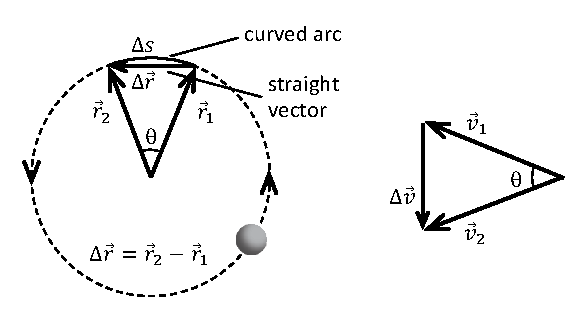
\includegraphics{circ_motion/circ_motion_fig3_new.eps} \par}
\vspace{0.3cm}

(b) Since the angles are the same and since the magnitudes of the position vectors 
never change (i.e., $r= r_{1}  = r_{2} $) and the magnitudes of the
velocities never change (i.e., $v = v_{1} = v_{2} $), use the properties
of similar triangles to explain why \( \frac{\Delta v}{v}=\frac{\Delta r}{r} \).
\vspace{20mm}

(c) Now use the equation in part (b) and the definition of $\langle
a\rangle$ to show that
\( \left\langle a_{c}\right\rangle =\frac{\Delta v}{\Delta t}=\frac{\left( \Delta r\right) }{\left( \Delta t\right) }\frac{v}{r}. \)
\vspace{20mm}

(d) The speed of the object as it rotates around the circle is 
given by \( v=\frac{\Delta s}{\Delta t} \).
Is the change in arc length, \( \Delta  s\), larger or smaller than the magnitude
of the change in the position vector, \( \Delta  r\)? Explain why the arc length
change and the change in the position vector are approximately the same when
$\Delta t$ is very small (so that the angle $\theta$ 
becomes very small) i.e., why is \( \Delta  s
\simeq  \Delta  r\)?
\vspace{20mm}

(e) If \( \Delta  s  \simeq   \Delta  r\), then what is the equation
for the speed in terms of \( \Delta  r\) and \( \Delta  t\)?  (Start with the formula for $v$ 
in part (d).)
\vspace{20mm}

(f) Using the equation in part (c), and your result from part (e), 
show that as \( \Delta  t\rightarrow 0 \), 
the instantaneous value of the centripetal acceleration is given by Eq. 1.

